\documentclass[a4paper,12pt]{article}

\usepackage{float}


\usepackage[utf8]{inputenc}
\usepackage[dvips]{graphicx}
%\usepackage{a4wide}
\usepackage{epsfig}
\usepackage{fancybox}
\usepackage{verbatim}
\usepackage{array}
\usepackage{latexsym}
\usepackage{alltt}
\usepackage{amssymb}
\usepackage{amsmath,amsthm}
\usepackage{bm}
\usepackage{wasysym}

%\usepackage{fullpage}
%\usepackage{hyperref}
\usepackage{listings}
\usepackage{color}
\usepackage{algorithm}
\usepackage{algpseudocode}
\usepackage[hmargin=2cm,vmargin=3.0cm]{geometry}
%\topmargin=0cm
%\topmargin=-1.8cm
%\addtolength{\textheight}{6.5cm}
%\addtolength{\textwidth}{2.0cm}
%\setlength{\leftmargin}{-3cm}
%\setlength{\oddsidemargin}{0.0cm}
%\setlength{\evensidemargin}{0.0cm}

%misc libraries goes here
\usepackage{tikz}
\usepackage{tikz-qtree}
\usetikzlibrary{automata,positioning}

\usepackage{multicol}
\usepackage{enumitem}

\usepackage[most]{tcolorbox}

\usepackage[colorlinks=true,urlcolor=black,linkcolor=black]{hyperref}


\lstdefinestyle{customtex}{
    %backgroundcolor=\color{lbcolor},
    tabsize=2,
    language=TeX,
    numbers=none,
    basicstyle=\footnotesize\ttfamily,
    numberstyle=\footnotesize,
    aboveskip={0.0\baselineskip},
    belowskip={0.0\baselineskip},
    %
    columns=flexible,
    keepspaces=true,
    fontadjust=true,
    upquote=true,
    %
    breaklines=true,
    prebreak=\raisebox{0ex}[0ex][0ex]{\ensuremath{\hookleftarrow}},
    frame=single,
    showtabs=false,
    showspaces=false,
    showstringspaces=false,
    %
    %identifierstyle=\color[rgb]{0,0.2,0.8},
    identifierstyle=\color[rgb]{0,0,0.5},
    %identifierstyle=\color[rgb]{0.133,0.545,0.133},
    %keywordstyle=\color[rgb]{0.8,0,0},
    %keywordstyle=\color[rgb]{0.133,0.545,0.133},
    keywordstyle=\color[rgb]{0,0,0.5},
    %commentstyle=\color[rgb]{0.133,0.545,0.133},
    commentstyle=\color[rgb]{0.545,0.545,0.545},
    %stringstyle=\color[rgb]{0.827,0.627,0.133},
    stringstyle=\color[rgb]{0.133,0.545,0.133},
    %
    literate={â}{{\^{a}}}1 {Â}{{\^{A}}}1 {ç}{{\c{c}}}1 {Ç}{{\c{C}}}1 {ğ}{{\u{g}}}1 {Ğ}{{\u{G}}}1 {ı}{{\i}}1 {İ}{{\.{I}}}1   {ö}{{\"o}}1 {Ö}{{\"O}}1 {ş}{{\c{s}}}1 {Ş}{{\c{S}}}1 {ü}{{\"u}}1 {Ü}{{\"U}}1 {~}{$\sim$}{1}
}

\lstdefinestyle{output}{
    %backgroundcolor=\color{lbcolor},
    tabsize=2,
    numbers=none,
    basicstyle=\footnotesize\ttfamily,
    numberstyle=\footnotesize,
    aboveskip={0.0\baselineskip},
    belowskip={0.0\baselineskip},
    %
    columns=flexible,
    keepspaces=true,
    fontadjust=true,
    upquote=true,
    %
    breaklines=true,
    prebreak=\raisebox{0ex}[0ex][0ex]{\ensuremath{\hookleftarrow}},
    frame=single,
    showtabs=false,
    showspaces=false,
    showstringspaces=false,
    %
    %identifierstyle=\color[rgb]{0.44,0.12,0.1},
    identifierstyle=\color[rgb]{0,0,0},
    keywordstyle=\color[rgb]{0,0,0},
    commentstyle=\color[rgb]{0,0,0},
    stringstyle=\color[rgb]{0,0,0},
    %
    literate={â}{{\^{a}}}1 {Â}{{\^{A}}}1 {ç}{{\c{c}}}1 {Ç}{{\c{C}}}1 {ğ}{{\u{g}}}1 {Ğ}{{\u{G}}}1 {ı}{{\i}}1 {İ}{{\.{I}}}1   {ö}{{\"o}}1 {Ö}{{\"O}}1 {ş}{{\c{s}}}1 {Ş}{{\c{S}}}1 {ü}{{\"u}}1 {Ü}{{\"U}}1
}

\lstset{style=customtex}


\tikzset{%
    terminal/.style={draw, rectangle,
    				 align=center, 
					 minimum height=1cm, 
					 minimum width=2cm,
					 fill=black!10,
					 anchor=mid},
    nonterminal/.style={draw, rectangle,
    					align=left,
					    minimum height=1cm, 
						minimum width=2cm, 
						anchor=mid},% and so on
}

%% Style for terminals
%\tikzstyle{terminal}=[draw, rectangle, 
%					  minimum height=1cm, 
%					  minimum width=2cm, 
%					  fill=black!20,
%					  anchor=south west]
%% Style for nonterminals
%\tikzstyle{nonterminal}=[draw, rectangle, 
%						 minimum height=1 cm, 
%						 minimum width=2 cm, 
%						 anchor=north east]


\newcommand{\HRule}{\rule{\linewidth}{1mm}}
\newcommand{\kutu}[2]{\framebox[#1mm]{\rule[-2mm]{0mm}{#2mm}}}
\newcommand{\gap}{ \\[1mm] }

\newcommand{\Q}{\raisebox{1.7pt}{$\scriptstyle\bigcirc$}}
\newcommand{\minus}{\scalebox{0.35}[1.0]{$-$}}

\setlength{\fboxsep}{10pt}

\tcbsetforeverylayer{enhanced jigsaw, breakable, arc=0mm, boxrule=1pt, boxsep=5pt, after=\vspace{1em}, colback=white, colframe=black}

\newcolumntype{P}[1]{>{\centering\arraybackslash}p{#1}}

\setlength\parindent{0pt}

%\renewcommand\arraystretch{1.2}

\newenvironment{Tab}[1]
  {\def\arraystretch{1}\tabular{#1}}
  {\endtabular}

%%%%%%%%%%%%%%%%%%%%%%%%%%%%%%%%%%%%%%%%%%%%%%%%%%%%%%%%%%%%%%%%%%%%%%%%%%%%%%%%%%%%%%

\title{Formal Languages and Abstract Machines \\ Take Home Exam 2}
\author{Ahmet Dara VEFA \\ 2237899} % write your name and id
\date{} % do not write any date

%%%%%%%%%%%%%%%%%%%%%%%%%%%%%%%%%%%%%%%%%%%%%%%%%%%%%%%%%%%%%%%%%%%%%%%%%%%%%%%%%%%%%%

\begin{document}
\HRule\\
Middle East Technical University \hfill Department of Computer Engineering
{\let\newpage\relax\maketitle}
\HRule\\
\vspace{1cm}

%%%%%%%%%%%%%%%%%%%%%%%%%%%%%%%%%%%%%%%%%%%%%%%%%%%%%%%%%%%%%%%%%%%%%%%%%%%%%%%%%%%%%%

% Write your answers below the section tags
\section{Context-Free Grammars \hfill \normalfont{(10 pts)}}

\paragraph{a)} Give the rules of the Context-Free Grammars to recognize strings in the given languages where $\Sigma=\{a,b\}$ and $S$ is the start symbol. \\  

$L(G)=\{w \mid \;  w \in \Sigma^*;\; |w| \geq 3;\; $  \hfill \small{(2/10 pts)} \\
\hspace*{22mm} the first and the second from the last symbols of $w$ are the same$\}$ \\

\begin{tcolorbox}
$S-> aKaZ \ | \  bKbZ$
\\
$Z-> a \ | \ b$
\\
$K-> aK\ | \ bK \ | \ e $
% \vspace{1cm} % remove this after your answer
\end{tcolorbox}


$L(G)=\{w \mid \;  w \in \Sigma^*;\; $ the length of w is odd$\}$ \hfill \small{(2/10 pts)} \\

\begin{tcolorbox}
$S-> aC \ | \ bC$
\\
$C-> aaC \ | \ abC\ | \ bbC \ | \ baC \ | \ e$
%\vspace{1cm} % remove this after your answer
\end{tcolorbox}


$L(G)=\{w \mid \;  w \in \Sigma^*;\; n(w,a)=2\cdot n(w,b)\}$ where $n(w,x)$ is the number of $x$ symbols in $w$ \hfill \small{(3/10 pts)} \\

\begin{tcolorbox}
$S-> e \ | \ SaSaSbS \ | \ SaSbSaS \ | \ SbSaSaS$
%\vspace{1cm} % remove this after your answer
\end{tcolorbox}



\paragraph{b)} Find the set of strings recognized by the CFG rules given below:         \hfill \small{(3/10 pts)} \\


$S \to X \mid Y$ \\
$X \to aXb \mid A \mid B$ \\
$A \to aA \mid a$ \\
$B \to Bb \mid b$ \\
$Y \to CbaC$ \\
$C \to CC \mid a \mid b \mid \varepsilon$  \\

\begin{tcolorbox}
$L(G)=\{w|(w \in(a^kb^l, \ k\neq l)) \cup (w \in \Sigma^*ba \Sigma^*)\}$
%\vspace{1cm} % remove this after your answer
\end{tcolorbox}


\newpage
\section{Parse Trees and Derivations \hfill \normalfont{(20 pts)}}
Given the CFG below, provide parse trees for given sentences in \textbf{a} and \textbf{b}.\\

\begin{lstlisting}[style=output,mathescape=true]
S   $\to$ NP VP
VP  $\to$ V NP | V NP PP
PP  $\to$ P NP
NP  $\to$ N | D N | NP PP
V   $\to$ wrote | built | constructed
D   $\to$ a | an | the | my
N   $\to$ John | Mary | Jane | man | book | automata | pen | class
P   $\to$ in | on | by | with
\end{lstlisting}

\paragraph{a)} Jane constructed automata with a pen \hfill \small{(4/20 pts)} \\

\begin{tcolorbox}
\Tree [.S [.NP [.N Jane ] ][.VP [.V constructed ] [.NP [.N automata ] ] [.PP [.P with ][.NP [.D a ][.N pen ] ] ] ] ]
\Tree [.S [.NP [.N Jane ] ][.VP [.V constructed ] [.NP [.NP [.N automata ] ] [.PP [.P with ][.NP [.D a ] [.N pen ] ] ] ] ] ]
%\vspace{12cm} % remove this after your answer
\end{tcolorbox}
%[.VP [.V constructed] [.NP [.N automata]] [.PP [.P with][.NP [.D a][.N pen]]]]
\paragraph{b)} my book in the man built a Jane by a pen \hfill \small{(4/20 pts)} \\

\begin{tcolorbox}
\Tree [.S [.NP [.NP [.D my ][.N book ] ][.PP [.P in ][.NP [.D the ][.N man ] ] ] ][.VP [.V built ][.NP [.D a ][.N Jane ] ][.PP [.P by ][.NP [.D a ][.N pen ] ] ] ] ]

\Tree [.S [.NP [.NP [.D my ][.N book ] ][.PP [.P in ][.NP [.D the ][.N man ] ] ] ][.VP [.V built ][.NP [.NP [.D a ][.N Jane ] ][.PP [.P by ][.NP [.D a ][.N pen ] ] ] ] ] ]
%\vspace{60cm} % remove this after your answer
\end{tcolorbox}

\newpage

Given the CFG below, answer \textbf{c}, \textbf{d} and \textbf{e} \\

\begin{lstlisting}[style=output,mathescape=true]
S  $\to$ E
E  $\to$ E + T | E - T | T
T  $\to$ T * I | T / I | I
I  $\to$ 0 | 1 | 2 | 3 | 4 | 6 | 7 | 8 | 9
\end{lstlisting}

\paragraph{c)} Provide the left-most derivation of 7 - 4 * 3 step-by-step and plot the final parse \hfill \small{(4/20 pts)} \\
tree matching that derivation \\

\begin{tcolorbox}
$S=>E=>E-T=>T-T=>I-T=>7-T=>7-T*I=>7-I*I=>7-4*I=>7-4*3$

 \Tree [.S [.E [.E [.T [.I 7 ] ] ][- ][.T [.T [.I 4 ] ][* ][.I 3 ] ] ] ]
%\vspace{4cm} % remove this after your answer
\end{tcolorbox}



\paragraph{d)} Provide the right-most derivation of 7 - 4 * 3 step-by-step and plot the final parse \hfill \small{(4/20 pts)} \\
 tree matching that derivation \\
 
\begin{tcolorbox}
$S=>E=>E-T=>E-T*I=>E-T*3=>E-I*3=>E-4*3=>T-4*3=>I-4*3=>7-4*3$

 \Tree [.S [.E [.E [.T [.I 7 ] ] ][- ][.T [.T [.I 4 ] ][* ][.I 3 ] ] ] ]
%\vspace{40cm} % remove this after your answer
\end{tcolorbox}
\newpage

\paragraph{e)} Are the derivations in \textbf{c} and \textbf{d} in the same similarity class?  \hfill \small{(4/20 pts)} \\

\begin{tcolorbox}
 Yes, since they both give the same parse tree they are in the same similarity class.
%\vspace{1cm} % remove this after your answer
\end{tcolorbox}


\newpage
\section{Pushdown Automata \hfill \normalfont{(30 pts)}}

\paragraph{a)} 
Find the language recognized by the PDA given below \hfill \small{(5/30 pts)} \\

\begin{tikzpicture}[shorten >=1pt,node distance=3cm,on grid,auto]
\node[state,initial,initial text=] (q_0) {$q_0$};
\node[state] (q_1) [right=of q_0] {$q_1$};
\node[state] (q_2) [above right=of q_1] {$q_2$};
\node[state] (q_3) [below right=of q_1] {$q_3$};
\node[state,accepting](q_4) [right=of q_2] {$q_4$};
\node[state](q_5) [right=of q_3] {$q_5$};
\node[state,accepting](q_6) [right=of q_5] {$q_6$};
\path[->]

(q_0) edge node {$\varepsilon,\varepsilon \to \#$} (q_1)
(q_1) edge [loop below] node {$x,\varepsilon \to x$} (q_1)

%%
(q_1) edge node {$\varepsilon,\varepsilon \to \varepsilon$} (q_2)
(q_2) edge [loop above] node {$y,x \to \varepsilon$} (q_2)

(q_2) edge node {$\varepsilon,\# \to \varepsilon$} (q_4)
(q_4) edge [loop above] node {$z,\varepsilon \to \varepsilon$} (q_4)

%%%

(q_1) edge node {$\varepsilon,\varepsilon \to \varepsilon$} (q_3)
(q_3) edge [loop below] node {$y,\varepsilon \to \varepsilon$} (q_3)

(q_3) edge node {$\varepsilon,\varepsilon \to \varepsilon$} (q_5)
(q_5) edge [loop below] node {$z,x \to \varepsilon$} (q_5)

(q_5) edge node {$\varepsilon,\# \to \varepsilon$} (q_6)
;
\end{tikzpicture} \\

\begin{minipage}{0.60\textwidth}
where the transition $((q_i,\alpha,\beta),(q_j,\gamma)) $ is represented as: 
\end{minipage}
\begin{minipage}{0.30\textwidth}
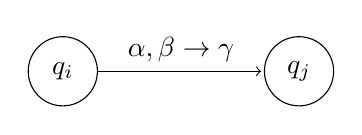
\begin{tikzpicture}[shorten >=1pt,node distance=3cm,on grid,auto]
\node[state] (q_i) {$q_i$};
\node[state] (q_j) [right=of q_i] {$q_j$};
\path[->]
(q_i) edge node {$\alpha,\beta \to \gamma$} (q_j);
\end{tikzpicture} \\
\end{minipage}


\begin{tcolorbox}
$L=\{ w|w \in (x^ny^mz^n \cup x^my^mz^n),(n,m \in N) \}$
%\vspace{2cm} % remove this after your answer
\end{tcolorbox}


\paragraph{b)} 
Design a PDA to recognize language $ L=\{x^n y^{m+n} x^m \mid \; n,m \geq 0; \; n,m \in \mathbb{N}  \} $  \hfill \small{(5/30 pts)} \\

\begin{tcolorbox}
\begin{center}
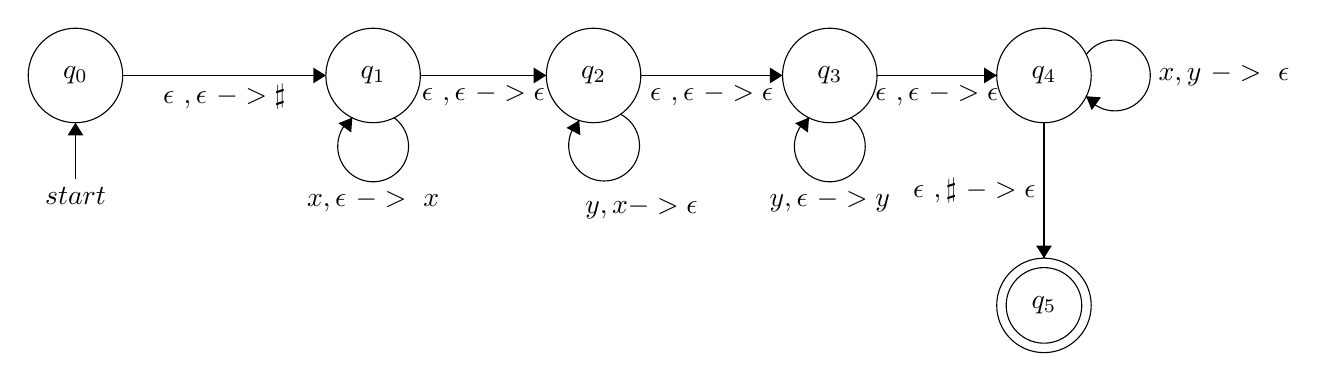
\begin{tikzpicture}[scale=0.2]
\tikzstyle{every node}+=[inner sep=0pt]
\draw [black] (3.2,-4.2) circle (3);
\draw (3.2,-4.2) node {$q_0$};
\draw [black] (22.1,-4.2) circle (3);
\draw (22.1,-4.2) node {$q_1$};
\draw [black] (36.1,-4.2) circle (3);
\draw (36.1,-4.2) node {$q_2$};
\draw [black] (51.1,-4.2) circle (3);
\draw (51.1,-4.2) node {$q_3$};
\draw [black] (64.7,-4.2) circle (3);
\draw (64.7,-4.2) node {$q_4$};
\draw [black] (64.7,-18.8) circle (3);
\draw (64.7,-18.8) node {$q_5$};
\draw [black] (64.7,-18.8) circle (2.4);
\draw [black] (3.2,-10.8) -- (3.2,-7.2);
\draw (3.2,-11.3) node [below] {$start$};
\fill [black] (3.2,-7.2) -- (2.7,-8) -- (3.7,-8);
\draw [black] (6.2,-4.2) -- (19.1,-4.2);
\fill [black] (19.1,-4.2) -- (18.3,-3.7) -- (18.3,-4.7);
\draw (12.65,-4.7) node [below] {$\epsilon\mbox{ },\epsilon\mbox{ }->\sharp$};
\draw [black] (23.423,-6.88) arc (54:-234:2.25);
\draw (22.1,-11.45) node [below] {$x,\epsilon\mbox{ }->\mbox{ }x$};
\fill [black] (20.78,-6.88) -- (19.9,-7.23) -- (20.71,-7.82);
\draw [black] (25.1,-4.2) -- (33.1,-4.2);
\fill [black] (33.1,-4.2) -- (32.3,-3.7) -- (32.3,-4.7);
\draw (29.1,-4.7) node [below] {$\epsilon\mbox{ },\epsilon\mbox{ }->\epsilon$};
\draw [black] (37.805,-6.654) arc (62.53077:-225.46923:2.25);
\draw (39.14,-11.89) node [below] {$y,x->\epsilon$};
\fill [black] (35.19,-7.05) -- (34.38,-7.53) -- (35.26,-7.99);
\draw [black] (39.1,-4.2) -- (48.1,-4.2);
\fill [black] (48.1,-4.2) -- (47.3,-3.7) -- (47.3,-4.7);
\draw (43.6,-4.7) node [below] {$\epsilon\mbox{ },\epsilon\mbox{ }->\epsilon$};
\draw [black] (52.423,-6.88) arc (54:-234:2.25);
\draw (51.1,-11.45) node [below] {$y,\epsilon\mbox{ }->y$};
\fill [black] (49.78,-6.88) -- (48.9,-7.23) -- (49.71,-7.82);
\draw [black] (54.1,-4.2) -- (61.7,-4.2);
\fill [black] (61.7,-4.2) -- (60.9,-3.7) -- (60.9,-4.7);
\draw (57.9,-4.7) node [below] {$\epsilon\mbox{ },\epsilon\mbox{ }->\epsilon$};
\draw [black] (67.38,-2.877) arc (144:-144:2.25);
\draw (71.95,-4.2) node [right] {$x,y\mbox{ }->\mbox{ }\epsilon$};
\fill [black] (67.38,-5.52) -- (67.73,-6.4) -- (68.32,-5.59);
\draw [black] (64.7,-7.2) -- (64.7,-15.8);
\fill [black] (64.7,-15.8) -- (65.2,-15) -- (64.2,-15);
\draw (64.2,-11.5) node [left] {$\epsilon\mbox{ },\sharp\mbox{ }->\epsilon$};
\end{tikzpicture}
\end{center}
%\vspace{3cm} % remove this after your answer
\end{tcolorbox}

\newpage

\paragraph{c)} 
Design a PDA to recognize language $ L=\{x^n y^m \mid \; n < m \leq 2n; \; n,m \in \mathbb{N^+} \} $  \hfill \small{(10/30 pts)} \\
Do not use multi-symbol push/pop operations in your transitions. \\
Simulate the PDA on strings \textit{xxy} (with only one rejecting derivation) and \textit{xxyyyy} (accepting derivation) with transition tables. \\

\begin{tcolorbox}
\begin{center}
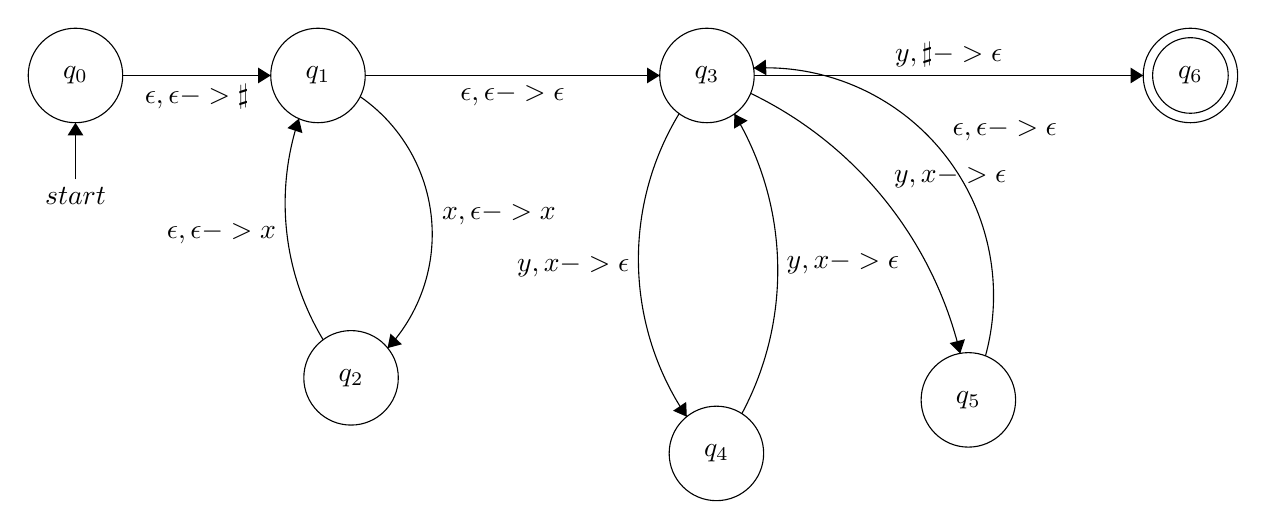
\begin{tikzpicture}[scale=0.2]
\tikzstyle{every node}+=[inner sep=0pt]
\draw [black] (3.3,-3.5) circle (3);
\draw (3.3,-3.5) node {$q_0$};
\draw [black] (18.7,-3.5) circle (3);
\draw (18.7,-3.5) node {$q_1$};
\draw [black] (20.8,-22.7) circle (3);
\draw (20.8,-22.7) node {$q_2$};
\draw [black] (43.4,-3.5) circle (3);
\draw (43.4,-3.5) node {$q_3$};
\draw [black] (44,-27.5) circle (3);
\draw (44,-27.5) node {$q_4$};
\draw [black] (60,-24.1) circle (3);
\draw (60,-24.1) node {$q_5$};
\draw [black] (74.1,-3.5) circle (3);
\draw (74.1,-3.5) node {$q_6$};
\draw [black] (74.1,-3.5) circle (2.4);
\draw [black] (3.3,-10.1) -- (3.3,-6.5);
\draw (3.3,-10.6) node [below] {$start$};
\fill [black] (3.3,-6.5) -- (2.8,-7.3) -- (3.8,-7.3);
\draw [black] (6.3,-3.5) -- (15.7,-3.5);
\fill [black] (15.7,-3.5) -- (14.9,-3) -- (14.9,-4);
\draw (11,-4) node [below] {$\epsilon ,\epsilon ->\sharp$};
\draw [black] (21.373,-4.84) arc (55.30378:-42.81995:10.636);
\fill [black] (23.12,-20.81) -- (24.03,-20.57) -- (23.3,-19.89);
\draw (26.54,-12.32) node [right] {$x,\epsilon ->x$};
\draw [black] (19.029,-20.283) arc (-148.88743:-198.62875:16.792);
\fill [black] (17.49,-6.24) -- (16.76,-6.84) -- (17.71,-7.16);
\draw (16.06,-13.54) node [left] {$\epsilon ,\epsilon ->x$};
\draw [black] (21.7,-3.5) -- (40.4,-3.5);
\fill [black] (40.4,-3.5) -- (39.6,-3) -- (39.6,-4);
\draw (31.05,-4) node [below] {$\epsilon ,\epsilon ->\epsilon$};
\draw [black] (42.116,-25.17) arc (-145.86171:-211.2741:17.818);
\fill [black] (42.12,-25.17) -- (42.08,-24.23) -- (41.25,-24.79);
\draw (38.51,-15.62) node [left] {$y,x->\epsilon$};
\draw [black] (45.139,-5.941) arc (31.01771:-28.15351:19.283);
\fill [black] (45.14,-5.94) -- (45.12,-6.88) -- (45.98,-6.37);
\draw (48.43,-15.39) node [right] {$y,x->\epsilon$};
\draw [black] (46.175,-4.635) arc (64.28574:13.43975:24.699);
\fill [black] (59.48,-21.15) -- (59.78,-20.25) -- (58.81,-20.49);
\draw (55.25,-9.96) node [right] {$y,x->\epsilon$};
\draw [black] (46.358,-3.033) arc (93.03854:-15.31305:14.474);
\fill [black] (46.36,-3.03) -- (47.18,-3.49) -- (47.13,-2.49);
\draw (58.96,-6.98) node [right] {$\epsilon ,\epsilon ->\epsilon$};
\draw [black] (46.4,-3.5) -- (71.1,-3.5);
\fill [black] (71.1,-3.5) -- (70.3,-3) -- (70.3,-4);
\draw (58.75,-3) node [above] {$y,\sharp ->\epsilon$};
\end{tikzpicture}
\end{center}
%\vspace{19cm} % remove this after your answer
\end{tcolorbox}

\paragraph{d)} Given two languages $L'$ and $L$ as $L'=\{w \mid \; w\in L; \; |w|=4n+2 \; for\; n\in \mathbb{N} \}$
\hfill \small{(10/30 pts)} \\
If $L$ is a CFL, show that $L'$ is also a CFL by constructing an automaton for $L'$ in terms of another automaton that recognizes $L$. \\

\begin{tcolorbox}

\begin{center}
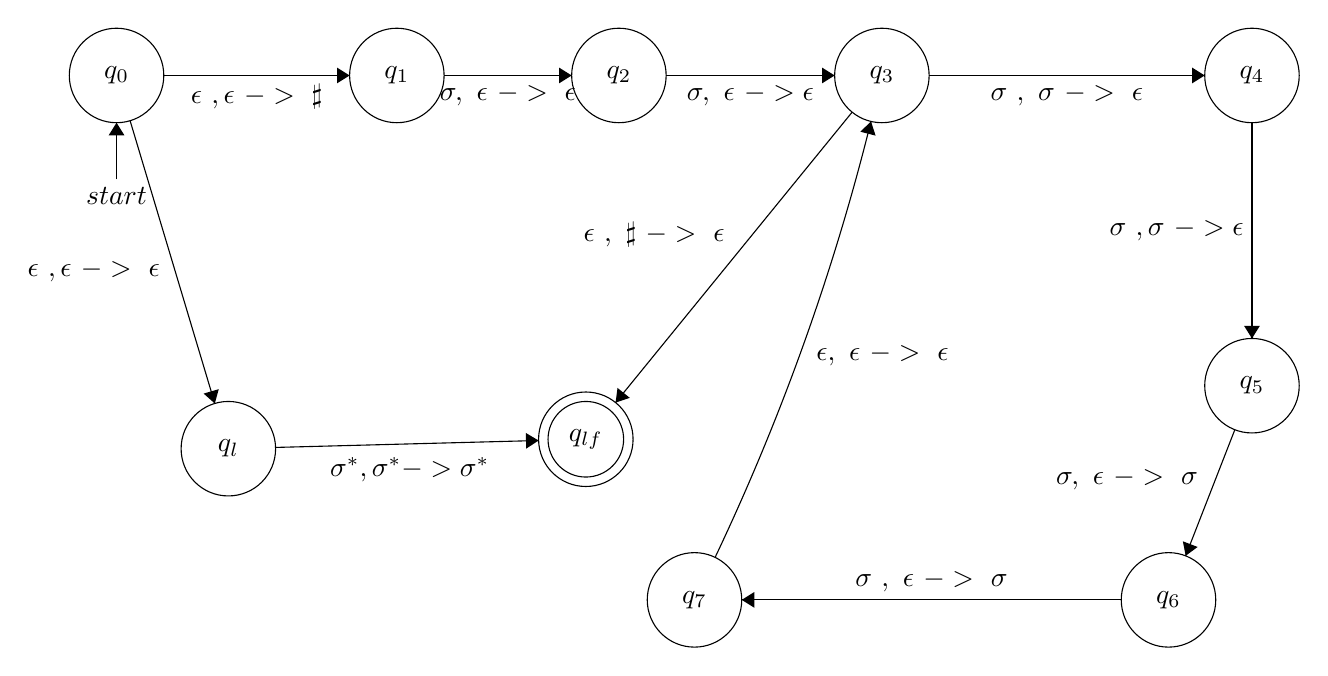
\begin{tikzpicture}[scale=0.2]
\tikzstyle{every node}+=[inner sep=0pt]
\draw [black] (4.2,-4.2) circle (3);
\draw (4.2,-4.2) node {$q_0$};
\draw [black] (22,-4.2) circle (3);
\draw (22,-4.2) node {$q_1$};
\draw [black] (36.1,-4.2) circle (3);
\draw (36.1,-4.2) node {$q_2$};
\draw [black] (52.8,-4.2) circle (3);
\draw (52.8,-4.2) node {$q_3$};
\draw [black] (76.3,-4.2) circle (3);
\draw (76.3,-4.2) node {$q_4$};
\draw [black] (11.3,-27.9) circle (3);
\draw (11.3,-27.9) node {$q_l$};
\draw [black] (34,-27.3) circle (3);
\draw (34,-27.3) node {$q_{lf}$};
\draw [black] (34,-27.3) circle (2.4);
\draw [black] (76.3,-23.9) circle (3);
\draw (76.3,-23.9) node {$q_5$};
\draw [black] (71,-37.5) circle (3);
\draw (71,-37.5) node {$q_6$};
\draw [black] (40.9,-37.5) circle (3);
\draw (40.9,-37.5) node {$q_7$};
\draw [black] (4.2,-10.8) -- (4.2,-7.2);
\draw (4.2,-11.3) node [below] {$start$};
\fill [black] (4.2,-7.2) -- (3.7,-8) -- (4.7,-8);
\draw [black] (5.06,-7.07) -- (10.44,-25.03);
\fill [black] (10.44,-25.03) -- (10.69,-24.12) -- (9.73,-24.4);
\draw (6.98,-16.65) node [left] {$\epsilon\mbox{ },\epsilon\mbox{ }->\mbox{ }\epsilon$};
\draw [black] (14.3,-27.82) -- (31,-27.38);
\fill [black] (31,-27.38) -- (30.19,-26.9) -- (30.21,-27.9);
\draw (22.82,-28.41) node [below] {$\sigma^*,\sigma^*->\sigma^*$};
\draw [black] (7.2,-4.2) -- (19,-4.2);
\fill [black] (19,-4.2) -- (18.2,-3.7) -- (18.2,-4.7);
\draw (13.1,-4.7) node [below] {$\epsilon\mbox{ },\epsilon\mbox{ }->\mbox{ }\sharp$};
\draw [black] (25,-4.2) -- (33.1,-4.2);
\fill [black] (33.1,-4.2) -- (32.3,-3.7) -- (32.3,-4.7);
\draw (29.05,-4.7) node [below] {$\sigma,\mbox{ }\epsilon\mbox{ }->\mbox{ }\epsilon$};
\draw [black] (39.1,-4.2) -- (49.8,-4.2);
\fill [black] (49.8,-4.2) -- (49,-3.7) -- (49,-4.7);
\draw (44.45,-4.7) node [below] {$\sigma,\mbox{ }\epsilon\mbox{ }->\epsilon$};
\draw [black] (50.91,-6.53) -- (35.89,-24.97);
\fill [black] (35.89,-24.97) -- (36.79,-24.67) -- (36.01,-24.04);
\draw (42.84,-14.32) node [left] {$\epsilon\mbox{ },\mbox{ }\sharp\mbox{ }->\mbox{ }\epsilon$};
\draw [black] (55.8,-4.2) -- (73.3,-4.2);
\fill [black] (73.3,-4.2) -- (72.5,-3.7) -- (72.5,-4.7);
\draw (64.55,-4.7) node [below] {$\sigma\mbox{ },\mbox{ }\sigma\mbox{ }->\mbox{ }\epsilon$};
\draw [black] (76.3,-7.2) -- (76.3,-20.9);
\fill [black] (76.3,-20.9) -- (76.8,-20.1) -- (75.8,-20.1);
\draw (75.8,-14.05) node [left] {$\sigma\mbox{ },\sigma\mbox{ }->\epsilon$};
\draw [black] (75.21,-26.7) -- (72.09,-34.7);
\fill [black] (72.09,-34.7) -- (72.85,-34.14) -- (71.91,-33.78);
\draw (72.9,-29.84) node [left] {$\sigma,\mbox{ }\epsilon\mbox{ }->\mbox{ }\sigma$};
\draw [black] (68,-37.5) -- (43.9,-37.5);
\fill [black] (43.9,-37.5) -- (44.7,-38) -- (44.7,-37);
\draw (55.95,-37) node [above] {$\sigma\mbox{ },\mbox{ }\epsilon\mbox{ }->\mbox{ }\sigma$};
\draw [black] (52.107,-7.119) arc (-13.93765:-25.3918:147.304);
\fill [black] (52.11,-7.12) -- (51.43,-7.77) -- (52.4,-8.02);
\draw (48.61,-21.98) node [right] {$\epsilon,\mbox{ }\epsilon\mbox{ }->\mbox{ }\epsilon$};
\end{tikzpicture}
\end{center}


Where $\sigma$ is the alphabet of L, $q_l$ is the starting node of L, $q_{lf}$ is the finish node of L



%\vspace{8cm} % remove this after your answer
\end{tcolorbox}






\newpage
\section{Closure Properties \hfill \normalfont{(20 pts)}}

Let $L_1$ and $L_2$ be context-free languages which are not regular, and let $L_3$ be a regular language. Determine whether the following languages are necessarily CFLs or not. If they need to be context-free, explain your reasoning. If not, give one example where the language is a CFL and a counter example where the language is not a CFL. \\

\paragraph{a)} $L_4 = L_1 \cap (L_2 \setminus L_3)$ \hfill \small{(10/20 pts)} \\

\begin{tcolorbox}
Let$L_6=L_2 - L_3=L_2 \cap \bar L_3$ \\ intersection of a non regular CF language and the complement of a regular language is CF language. \\
$L_1 \cap L_6$ is the intersection of 2 CF languages. Since CF languages are not closed under intersection $L_4$ can be either non-CF:\\
let $L_1=\{ a^nb^nc^m:m,n \in N \}$\\
let $L_2 \cap \bar L_3 = \{ a^mb^nc^n: m,n\in N \}$
$L_4$ is not-CF.
\\
or it can be CF: \\
let $L_1=\{ a^nb^n:n \in N\}$\\
let $L_2=\{ a^nb^n:n \in N\}$\\
let $L_3=\{ \}$\\
so  $L_2 \cap \bar L_3=L_2=L_1$, therefore $L_5=L_1 \cap L_2=\{ a^nb^n:n \in N\} $. \\
So $L_5$ is CF.

%\vspace{6cm} % remove this after your answer
\end{tcolorbox}

\paragraph{b)} $L_5 = (L_1 \cap L_3)\text{*}$ \hfill \small{(10/20 pts)} \\

\begin{tcolorbox}
$(L_1 \cap L_2)^*$ is always CF since $(L_1 \cap L_2)$ can be anything from $\{ \}$ to a CF language, which makes it a CF language($RL \subseteq CFL $). CF languages are closed under kleene star(Theorem 3.5.1), so $L_5$ is context free.
%\vspace{6cm} % remove this after your answer
\end{tcolorbox}





\newpage
\section{Pumping Theorem \hfill \normalfont{(20 pts)}}

\paragraph{a)} Show that $L=\{a^n m^n t^i \mid \; n\leq i \leq 2n\}$ is not a Context Free Language \hfill \small{(10/20 pts)} \\
using Pumping Theorem for CFLs. \\

\begin{tcolorbox}
Assume L is a CFL. Then for some $w=a^km^kt^{2k}$, where K is the pumping length. By the Pumping Theorem, there exists a split $w=uvxyz$ st. $\mid vxy \mid < K \ and \ \mid vy \mid\geq 1$.\\
There are 5 cases.\\
First one is where vxy is all taken from $a^k$ .\\
Second one is where vxy is all taken from $m^k$ .\\
Third one is where vxy is all taken from $t^{2k}$ .\\
Fourth one is where vxy is taken from $a^km^k$.\\
Fifth one is where vxy is taken from $m^kt^{2k}$.\\
For cases 1 and 2: vxy consists of a's or m's. If we pump vxy for i=2 we get $w'=a^lm^jt^{2k}$ where $l \neq j$. This is a contradiction with the $w=a^km^kt^{2k}$.\\
For case 3: vxy consists of t's. If we pump vxy for i=2 we get $w'=a^km^kt^j$ where j>2k.This is a contradiction with the $w=a^km^kt^{2k}$.\\
For case 4: vxy consists of a's and m's. If we pump vxy for i=0, we get $w'=a^jm^pt^{2k}$ where either $j \neq p$ or 2j<2k.This is a contradiction with the $w=a^km^kt^{2k}$.\\
For case 5: vxy consists of m's and t's.If we pump vxy for i=2 we get $w'=a^km^jt^l$ where either $k \neq j$ or $l > 2k$.This is a contradiction with the $w=a^km^kt^{2k}$.\\
So by pumping theorem this language is not CF.
%\vspace{8cm} % remove this after your answer
\end{tcolorbox}


\paragraph{b)} Show that $L=\{a^n b^{2n} a^n \mid \; n \in \mathbb{N+} \}$ is not a Context Free Language \hfill \small{(10/20 pts)} \\
using Pumping Theorem for CFLs. \\

\begin{tcolorbox}
Assume L is a CFLç Then for some $w=a^kb^{2k}a^k$, where k is the pumping length. By the pumping theorem, there exists a split$w=uvxyz$ st. $\mid vxy \mid < K \ and \ \mid vy \mid\geq 1$.\\
There are 5 cases.\\
First one is where vxy is all taken from $a^k$ .\\
Second one is where vxy is all taken from $b^{2k}$ .\\
Third one is where vxy is all taken from $a^{k}$ .\\
Fourth one is where vxy is taken from $a^kb^{2k}$.\\
Fifth one is where vxy is taken from $b^{2k}a^k$.\\
For cases 1,2 and 3: vxy consists of a's or b's. If we pump vxy for i=0 we get $w'=a^pb^ra^s$ where either $p \neq s$ or $r \neq 2p$ or $r \neq 2s$. This is a contradiction with the $w=a^kb^{2k}a^k$.\\
For cases 4 and 5: vxy consists of a's and b's. If we pump vsy for i=0, we get $w'=a^pb^ra^s$  where either $p \neq s$ or $r \neq 2p$ or $r \neq 2s$. This is a contradiction with the $w=a^kb^{2k}a^k$.\\
So by pumping theorem this language is not CF. 
\vspace{8cm} % remove this after your answer
\end{tcolorbox}





\newpage
\section{CNF and CYK \hfill \normalfont{(not graded)}}

\paragraph{a)} Convert the given context-free grammar to Chomsky Normal Form. \\

$ S   \to XSX \mid xY $ \\
$ X   \to Y \mid S $ \\
$ Y   \to z \mid \varepsilon $ \\

\begin{tcolorbox}
answer here ...
\vspace{18cm} % remove this after your answer
\end{tcolorbox}


\paragraph{b)} Use the grammar below to parse the given sentence using Cocke–Younger–Kasami algorithm. \\
Plot the parse trees. \\

\begin{multicols}{2}
S $\to$ NP VP \\
S $\to$ X1 VP \\
X1 $\to$ Aux NP \\
S $\to$ book $\mid$ include $\mid$ prefer \\
S $\to$ Verb NP \\
S $\to$ X2 PP \\
S $\to$ Verb PP \\
S $\to$ VP PP \\
NP $\to$ I $\mid$ she $\mid$ me $\mid$ Houston \\
NP $\to$ Det Nom \\
Nom $\to$ book $\mid$ flight $\mid$ meal $\mid$ money \\
Nom $\to$ Nom Noun \\
Nom $\to$ Nom PP \\
VP $\to$ book $\mid$ include $\mid$ prefer \\
VP $\to$ Verb NP \\
VP $\to$ X2 PP \\
X2 $\to$ Verb NP \\
VP $\to$ Verb PP \\
VP $\to$ VP PP \\
PP $\to$ Prep NP \\
Det $\to$ that $\mid$ this $\mid$ the $\mid$ a \\
Noun $\to$ book $\mid$ flight $\mid$ meal $\mid$ money \\
Verb $\to$ book $\mid$ include $\mid$ prefer \\
Aux $\to$ does \\
Prep $\to$ from $\mid$ to $\mid$ on $\mid$ near $\mid$ through \\
\end{multicols}

\vspace{5mm}

book the flight through Houston \\

\begin{tcolorbox}

\scriptsize

Empty parse table:\\
\begin{tikzpicture}[node distance=0cm, outer sep = 0pt]

\node[terminal] (l0) {
    \begin{tabular}{@{}P{2.9cm}|@{}P{2.9cm}|@{}P{2.9cm}|@{}P{2.9cm}|@{}P{2.9cm}}
    book & the & flight & through & Houston \\
    \end{tabular}
};

\node[nonterminal] (l1) [above = of l0] {
    \begin{tabular}{@{}P{2.9cm}|@{}P{2.9cm}|@{}P{2.9cm}|@{}P{2.9cm}|@{}P{2.9cm}}
    1:1 & 
    2:2 & 
    3:3 & 
    4:4 & 
    5:5 \\
    \end{tabular}
};

\node[nonterminal] (l2) [above = of l1.north] {
    \begin{tabular}{@{}P{2.9cm}|@{}P{2.9cm}|@{}P{2.9cm}|@{}P{2.9cm}}
    1:2 $\to$ 1:1 2:2 & 
    2:3 $\to$ 2:2 3:3 & 
    3:4 $\to$ 3:3 4:4 & 
    4:5 $\to$ 4:4 5:5 \\
    \end{tabular}
};

\node[nonterminal] (l3) [above = of l2.north] {
    \begin{tabular}{@{}P{2.9cm}|@{}P{2.9cm}|@{}P{2.9cm}}
        \begin{tabular}{@{}l} 1:3 $\to$ 1:1 2:3 \\ 1:3 $\to$ 1:2 3:3 \end{tabular}& 
        \begin{tabular}{@{}l} 2:4 $\to$ 2:2 3:4 \\ 2:4 $\to$ 2:3 4:4 \end{tabular}& 
        \begin{tabular}{@{}l} 3:5 $\to$ 3:3 4:5 \\ 3:5 $\to$ 3:4 5:5 \end{tabular}\\
    \end{tabular}
};

\node[nonterminal] (l4) [above = of l3.north] {
    \begin{tabular}{@{}P{2.9cm}|@{}P{2.9cm}}
        \begin{tabular}{@{}l}1:4 $\to$ 1:1 2:4 \\ 1:4 $\to$ 1:2 3:4 \\ 1:4 $\to$ 1:3 4:4 \end{tabular}& 
        \begin{tabular}{@{}l}2:5 $\to$ 2:2 3:5 \\ 2:5 $\to$ 2:3 4:5 \\ 2:5 $\to$ 2:4 5:5 \end{tabular}\\
    \end{tabular}
};

\node[nonterminal] (l5) [above = of l4.north] {
    \begin{tabular}{@{}P{2.9cm}}
        \begin{tabular}{@{}l}
        1:5 $\to$ 1:1 2:5 \\ 1:5 $\to$ 1:2 3:5 \\ 
        1:5 $\to$ 1:3 4:5 \\ 1:5 $\to$ 1:4 5:5 
        \end{tabular}\\
    \end{tabular}
};

\end{tikzpicture}\\\\

rest of the answer here ...\\
\vspace{4cm} % remove this after your answer
\end{tcolorbox}



\newpage
\section{Deterministic Pushdown Automata \hfill \normalfont{(not graded)}}
Provide a DPDA to recognize the given languages, the DPDA must read its entire input and finish with an empty stack.
\paragraph{a)} $a^*bc \cup a^nb^nc$ \\

\begin{tcolorbox}
answer here ...
\vspace{12cm} % remove this after your answer
\end{tcolorbox}

\newpage

\paragraph{b)} $(aa)^*c \cup a^nb^nc$ \\

\begin{tcolorbox}
answer here ...
\vspace{12cm} % remove this after your answer
\end{tcolorbox}



\end{document}

​
